\documentclass[tikz,border=8pt]{standalone}
% Shared look for every TikZ diagram. Load with \input{../../tools/tikz-style.tex}
\usepackage[sfdefault]{roboto}
\usetikzlibrary{arrows.meta, positioning, shapes.geometric, calc, fit, backgrounds}
\definecolor{cblue}{HTML}{4C78A8}
\definecolor{corange}{HTML}{F58518}
\definecolor{cgreen}{HTML}{54A24B}
\definecolor{cred}{HTML}{E45756}
\definecolor{cpurple}{HTML}{B279A2}
\definecolor{cgrey}{HTML}{6B6B6B}
\tikzset{
  every picture/.style={font=\sffamily, line width=1.2pt},
  box/.style={draw=#1, fill=#1!12, rounded corners=4pt, align=center, inner sep=7pt, minimum height=1.1cm},
  box/.default=cgrey,
  arrow/.style={-{Stealth[length=3mm]}, draw=cgrey, line width=1.4pt},
  title/.style={font=\sffamily\bfseries\Large},
  note/.style={font=\sffamily\small, text=cgrey, align=center},
}
\AtBeginDocument{\hyphenpenalty=10000 \exhyphenpenalty=10000}

% The g2o graph TEB builds for a band of 4 poses (TebOptimalPlanner::buildGraph, ros2-master): vertices are the
% poses s1..s4 (s1 and s4 fixed) and the time steps dT1..dT3; each edge is one cost term and joins the vertices it
% reads. One edge of each kind is drawn; the code adds one per pose, piece or pair of pieces. Weights: teb_config.h.
\begin{document}
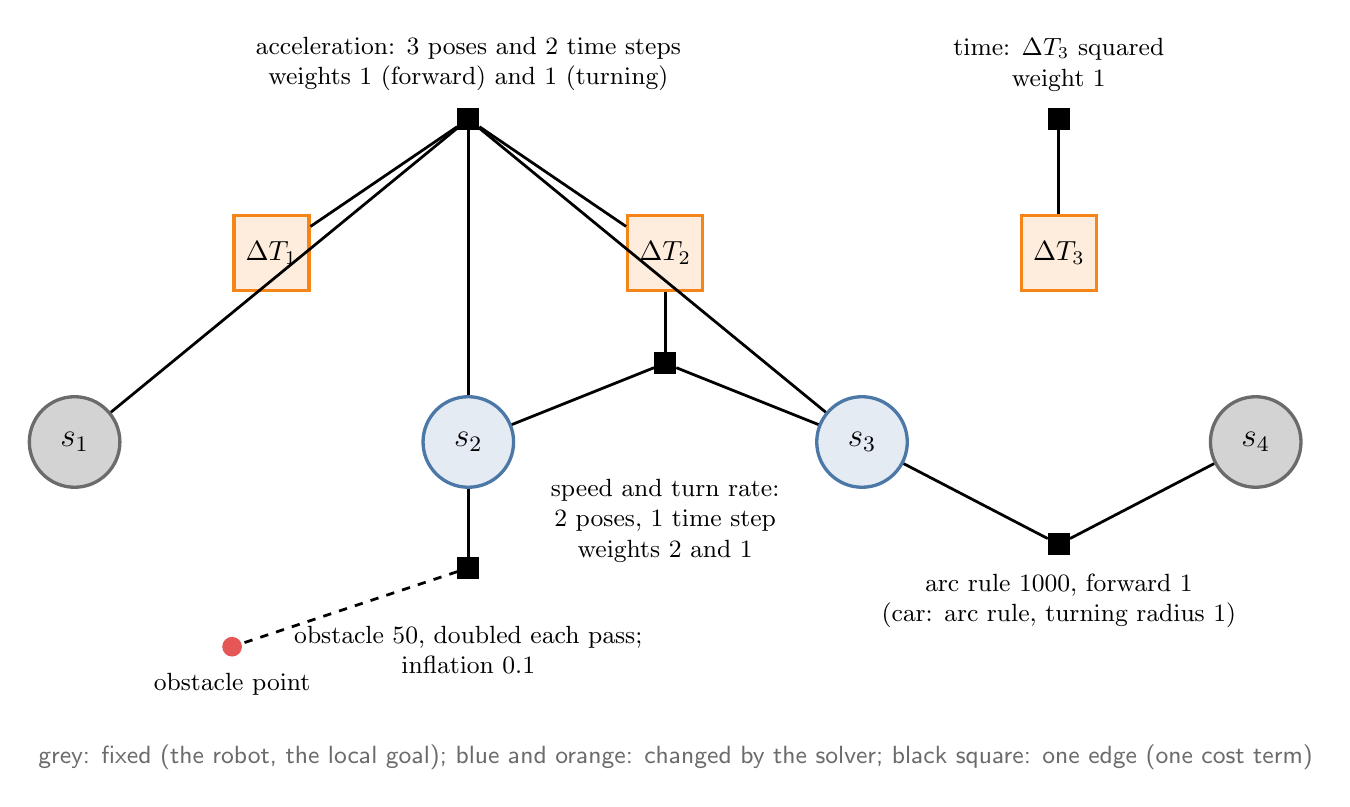
\begin{tikzpicture}[
  pose/.style={circle, draw=cblue, fill=cblue!15, minimum size=1.15cm, font=\large},
  fixed/.style={circle, draw=cgrey, fill=cgrey!30, minimum size=1.15cm, font=\large},
  dt/.style={rectangle, draw=corange, fill=corange!15, minimum size=0.95cm},
  edge/.style={rectangle, draw=black, fill=black, minimum size=0.24cm, inner sep=0pt},
  lab/.style={font=\small, align=center},
  link/.style={draw=black, line width=1pt}]
  \node[fixed] (s1) at (0,0) {$s_1$};
  \node[pose]  (s2) at (5,0) {$s_2$};
  \node[pose]  (s3) at (10,0) {$s_3$};
  \node[fixed] (s4) at (15,0) {$s_4$};
  \node[dt] (t1) at (2.5,2.4) {$\Delta T_1$};
  \node[dt] (t2) at (7.5,2.4) {$\Delta T_2$};
  \node[dt] (t3) at (12.5,2.4) {$\Delta T_3$};
  \node[edge] (eT) at (12.5,4.1) {};
  \draw[link] (eT) -- (t3);
  \node[lab, above=0.08cm of eT] {time: $\Delta T_3$ squared\\ weight 1};
  \node[edge] (eA) at (5,4.1) {};
  \foreach \v in {s1, s2, s3, t1, t2} \draw[link] (eA) -- (\v);
  \node[lab, above=0.08cm of eA] {acceleration: 3 poses and 2 time steps\\ weights 1 (forward) and 1 (turning)};
  \node[edge] (eV) at (7.5,1.0) {};
  \foreach \v in {s2, s3, t2} \draw[link] (eV) -- (\v);
  \node[lab] at (7.5,-1.0) {speed and turn rate:\\ 2 poses, 1 time step\\ weights 2 and 1};
  \node[edge] (eK) at (12.5,-1.3) {};
  \draw[link] (eK) -- (s3); \draw[link] (eK) -- (s4);
  \node[lab, below=0.1cm of eK] {arc rule 1000, forward 1\\ (car: arc rule, turning radius 1)};
  \node[circle, fill=cred, minimum size=0.25cm, inner sep=0pt] (ob) at (2.0,-2.6) {};
  \node[lab, below=0.05cm of ob] {obstacle point};
  \node[edge] (eO) at (5,-1.6) {};
  \draw[link] (eO) -- (s2); \draw[link, dashed] (eO) -- (ob);
  \node[lab, anchor=north] at (5,-2.2) {obstacle 50, doubled each pass;\\ inflation 0.1};
  \node[note, anchor=west] at (-0.6,-4.0) {grey: fixed (the robot, the local goal); blue and orange: changed by the solver; black square: one edge (one cost term)};
\end{tikzpicture}
\end{document}
